

\documentclass[a4paper,12pt,oneside]{book}

%---------
% packages
%---------
\usepackage[dvips]{graphicx}
\usepackage[T1]{fontenc}
\usepackage[utf8]{inputenc}
\usepackage[english]{babel}
\usepackage{color}
\usepackage[dvipsnames]{xcolor}
\usepackage{fancyhdr}
\usepackage{amsmath}
\usepackage{array}
\usepackage{colortbl}
\usepackage{amssymb}
\usepackage{fancybox}
\usepackage{float}
\usepackage{epic}
\usepackage{curves}
\usepackage{subfigure}
\usepackage{subeqnarray}
\usepackage{hyperref}
\usepackage{url}
\usepackage{lscape}
%\usepackage{lettrine}
%\usepackage{textcomp}
\usepackage{multicol}
\usepackage{caption}
\usepackage{wasysym}
%\usepackage{mathbx}
\usepackage{natbib}
\usepackage{ifpdf}
\usepackage{minitoc}
\usepackage{xspace}
\usepackage{doi}
\usepackage{times}
\usepackage{tikz}
\usepackage{listings}
\usepackage{makeidx}
\usepackage{booktabs}
\usepackage[explicit]{titlesec}
%\usepackage{texgraph}
\usepackage{epic,eepic}
\usepackage{rotating}
\usepackage{etex}

\lstdefinestyle{Bash}
{language=bash,
keywordstyle=\color{blue},
basicstyle=\ttfamily,
morekeywords={charles@gher13},
alsoletter={:~$},
commentstyle=\color{dkgreen},
morekeywords=[2]{charles@gher13:},
keywordstyle=[2]{\color{red}},
literate={\$}{{\textcolor{red}{\$}}}1 
         {:}{{\textcolor{red}{:}}}1
         {~}{{\textcolor{red}{\textasciitilde}}}1,
}
\lstset{
    breaklines     = true,
    frame          = single,
    rulecolor=     \color{gray},
}

%$

\lstdefinestyle{Matlab}
{language=matlab,
keywordstyle=\color{blue},
basicstyle=\ttfamily,
morekeywords={charles@gher13},
alsoletter={:~$},
commentstyle=\color{dkgreen},
morekeywords=[2]{charles@gher13:},
keywordstyle=[2]{\color{red}},
literate={\$}{{\textcolor{red}{\$}}}1 
         {:}{{\textcolor{red}{:}}}1
         {~}{{\textcolor{red}{\textasciitilde}}}1,
}
\lstset{
    breaklines     = true,
    frame          = single,
    rulecolor=     \color{gray},
}

%$

% paths + extensions for the figures
\DeclareGraphicsExtensions{.pdf,.jpg,.JPG,.png,.PNG}
\graphicspath{
{./figures/preprocessing/},{./figures/postprocessing/},{./figures/icones/},{./figures/test_cases/},
{./figures/examples/},{./figures/gallery/},{./figures/images/},{./figures/GUI/},{./figures/analysis/},
{./figures/errors/},{./figures/advection/},{./figures/papers/},{./figures/divaonweb/}
} 
 
%------------------------
%biblio style
%------------------------
\bibliographystyle{divagher}
%\bibliographystyle{plain}
% ------------------------------------------------
% NEW COLOR
\definecolor{gris}{rgb}{0.7,0.7,0.7}
\definecolor{darkgreen}{rgb}{0.14 0.73 0.21}

% ------------------------------------------------
% LENGTH DEFINITIONS
%-------------------------------------------------
\setlength{\textwidth}{16cm}
\setlength{\textheight}{24cm}
\setlength{\headheight}{50.3pt}
\setlength{\footskip}{45pt}
\setlength{\hoffset}{-1cm}
\setlength{\voffset}{-3cm}
\setlength{\unitlength}{1cm}
\setlength{\parindent}{0pt}
% ------------------------------------------------
% new commands
%-------------------------------------------------
\renewcommand{\footrulewidth}{0.4pt}
\renewcommand{\captionfont}{\it \small}

%\renewcommand{\LettrineFontHook}{\color[gray]{0.5}}

\newcommand{\example}{\underline{Example}:\,}
\newcommand{\examples}{\underline{Examples}:\,}
\newcommand{\be}{\begin{equation}}
\newcommand{\ee}{\end{equation}}
\newcommand{\beq}{\begin{eqnarray}}
\newcommand{\eeq}{\end{eqnarray}}
\newcommand{\beqn}{\begin{eqnarray*}}
\newcommand{\eeqn}{\end{eqnarray*}}

\newcommand{\montant}{\rule{0pt}{3ex}}
% ------------------------------------------------
% ABBREVIATION
%-------------------------------------------------

\newcommand{\diva}{\textsf{Diva}\xspace}
\newcommand{\matlab}{\textsf{Matlab}\xspace}
\newcommand{\plplot}{\textsf{PlPlot}}
\newcommand{\tcltk}{\textsf{Tcl/Tk}}
\newcommand{\divaversion}{4.3}
\newcommand{\gnuplot}{\textsf{gnuplot\xspace}}
\newcommand{\divawebpage}{http://modb.oce.ulg.ac.be/mediawiki/index.php/DIVA}

\newcommand{\question}{Why do I get this error?}
\newcommand{\answer}{How to solve it?}

% ------------------------------------------------
% JMB newcommands
%-------------------------------------------------

\newcommand{\nablab}{\boldsymbol{\nabla}}
\newcommand{\statmean}[1]{\left\langle #1 \right\rangle}
\newcommand{\mean}[1]{\statmean{#1}}
\newcommand{\true}[1]{{#1}^t}
\newcommand{\analyzed}[1]{{#1}^a}
\newcommand{\observation}{ \mbox{\boldmath   $ \protect\mathrm{y} $} }
\newcommand{\forecasted}[1]{{#1}^f}
\newcommand{\Hobs}{\matr{H}}
\newcommand{\errorv}{\vect{\epsilon}}
\newcommand{\errorobs}{\vect{\epsilon}^o}

\newcommand{\sing} {\rho}
\newcommand{\vnorm}[1] { \parallel \! #1 \! \parallel }
\newcommand{\taumax}[1] { \mu_{#1}^{max} }

\newcommand{\vecti}[1] { \mbox{\boldmath   $ \protect#1 $} }
\newcommand{\vects}[1] {{\boldsymbol {#1}}}
\newcommand{\vect}[1] {{\vec{#1}}}
\newcommand{\tens}[1] { \mbox{\boldmath   $ \protect\mathsf{#1} $} }
\newcommand{\matr}[1]{\mbox{$\mathbf{#1} $} }
\newcommand{\trcon}[1]{{#1}^\star}
\newcommand{\adj}[1]{\trcon{#1}}
\newcommand{\transp}[1]{{#1}^{\protect\mathrm{T}}}
\newcommand{\conj}[1]{\bar{#1}}
\newcommand{\inv}[1]{{#1}^{ \mbox{\small{-}}  1}}
\newcommand{\psinv}[1]{{#1}^{- \! \! \! 1}}
\newcommand{\noise}{\epsilon}
\newcommand{\signal}{\sigma}
\newcommand{\snr}{\lambda}

\newcommand{\ddiff}{\mbox{d}}
\newcommand{\diag}{\mbox{diag}}
\renewcommand{\vect}[1] { \mbox{\boldmath   $ #1 $} }
\renewcommand{\adj}[1]{{#1}^\mathsf{T}}
\renewcommand{\transp}[1]{{#1}^\mathsf{T}}
\renewcommand{\matr}[1] { \mbox{\boldmath   $ \protect\mathsf{#1} $} }
\renewcommand{\vect}[1] { \mbox{\boldmath   $ \protect\mathsf{#1} $} }
\newcommand{\posx}{\mathsf{r}}
\newcommand{\trace}[1]{\mathrm{trace}\left( #1 \right)}

\newcommand{\LaTeXPiX}[3]{
                          \begin{sidewaysfigure*}[ht]
                            \begin{center}
                            {\small{
                                \input{#1.eepic}
                                \caption{#2
                                \label{#3}}
                                }}
                            \end{center}
                          \end{sidewaysfigure*}
                        }
% ----------end of JMB newcommands

% ------------------------------------
% new kind of floating
%-------------------------------------
\floatstyle{boxed} 
\newfloat{exfile}{htbp}{exf}[chapter]
\floatname{exfile}{Example file}
% ------------------------------------------------

\newtheorem{tips}{Tips}[chapter]

\newcommand{\btips}{%\rule{1ex}{1ex}\,\,
\begin{tips}}
\newcommand{\etips}{\,\,\rule{1ex}{1ex}%
\end{tips}}

% level of diffuculty for the user
\newcommand{\beginer}{$\star$}
\newcommand{\intermediate}{$\star\star$}
\newcommand{\expert}{$\star\star\star$}

\newcommand{\directory}[1]{\texttt{\color{ForestGreen}{#1}}}
\newcommand{\file}[1]{\texttt{\color{MidnightBlue}{#1}}}
\newcommand{\command}[1]{\texttt{\color{RedOrange}{#1}}}

\def\BibTeX{{\rm B\kern-.05em{\sc i\kern-.025em b}\kern-.08em
    T\kern-.1667em\lower.7ex\hbox{E}\kern-.125emX}}
    
% ------------------------------------------------
% hyperref setup
%-------------------------------------------------
\hypersetup{bookmarksopen=true,
bookmarksnumbered=true,  
pdffitwindow=false, 
pdfstartview=FitP,
pdftoolbar=true,
pdfmenubar=true,
pdfwindowui=true,
pdfauthor={C.~Troupin, M.~Ouberdous, J.-M.~Beckers},
pdftitle={Diva User Guide},
pdfsubject={Geostatistics analysis tool},
bookmarksopenlevel=2,
colorlinks=true,%
breaklinks=true,%
colorlinks=true,%
linkcolor=blue,anchorcolor=blue,%
citecolor=blue,filecolor=blue,%
menucolor=black,%
urlcolor=blue}

% ------------------------------------------------
% page style
%-------------------------------------------------

\pagestyle{fancy} %Forces the page to use the fancy template
\renewcommand{\chaptermark}[1]{\markboth{\chaptername\ \MakeUppercase{\thechapter.\ #1}}{}}
\renewcommand{\sectionmark}[1]{\markright{\thesection.\ #1}}
%The text used in the header is determined by the arguments to the \markboth

\fancyhf{} %Clears all header and footer fields, in preparation.
\fancyhead[L]{\parbox{8cm}{\flushleft\textcolor{gris}{\leftmark}\\
\rule{\textwidth}{0pt}}}
\fancyhead[C]{\parbox{\textwidth}{\rule{0pt}{2.8ex}\\
\textcolor{gris}{\rule{\textwidth}{1pt}}}}
\fancyhead[R]{\parbox{6cm}{\flushright\textcolor{gris}{\rightmark}\\
\rule{\textwidth}{0pt}}} 
\renewcommand{\headrulewidth}{0pt} %Underlines the header. (Set to 0pt if not required).
\renewcommand{\footrulewidth}{0pt} %Underlines the footer. (Set to 0pt if not required)..
%\fancyfoot[C]{\large\bfseries \textcolor{gris}{--\thepage--} }

\fancyfoot[C]{\large\thepage}

% ------------------------------------------------
% chapter style
%-------------------------------------------------

\newcommand*\chapterlabel{}
\titleformat{\chapter}
  {\gdef\chapterlabel{}
   \normalfont\sffamily\Huge\bfseries\scshape}
  {\gdef\chapterlabel{\thechapter\ }}{0pt}
  {\begin{tikzpicture}[remember picture,overlay]
    \node[yshift=-2.5cm] at (current page.north west)
      {\begin{tikzpicture}[remember picture, overlay]
        \draw[fill=lightgray] (0,0) rectangle
          (\paperwidth,2.5cm);
        \node[anchor=east,xshift=.95\paperwidth,rectangle,
              rounded corners=20pt,inner sep=11pt,
              fill=black]
              {\color{white}\chapterlabel#1};
       \end{tikzpicture}
      };
   \end{tikzpicture}
  }
\titlespacing*{\chapter}{0pt}{50pt}{-60pt}
%%%%%%%%%%%%%%%%%%%%%%%%%%%%%%%%%%%%%%%%%%%%%%%%%%%%%%%%%%%%%%%

\parskip 0.25cm
\urlstyle{tt}

% ------------------------------------------------
%% Define a new 'leo' style for the package that will use a smaller font.
\makeatletter
\def\url@leostyle{%
  \@ifundefined{selectfont}{\def\UrlFont{\sf}}{\def\UrlFont{\small}}}
\makeatother
%% Now actually use the newly defined style.
\urlstyle{leo}

%-----------------------------------------------------
% For the title page
%-----------------------------------------------------

\newcommand{\HRule}[1]{\hfill \rule{0.2\linewidth}{#1}} 	% Horizontal rule

\definecolor{grey}{rgb}{0.9,0.9,0.9} 

\makeatletter							% Title
\def\printtitle{%						
    {\centering \@title\par}}
\makeatother									

\makeatletter							% Author
\def\printauthor{%					
    {\centering \large \@author}}				
\makeatother		


\title{\diva User Guide for EMODNET specials}
\author{C.~Troupin, M.~Ouberdous, D.~Sirjacobs, A.~Alvera-Azc\'{a}rate,\\ A.~Barth, M.-E. Toussaint, S.~Watelet \& J.-M.~Beckers}
\date{}

\makeindex


\begin{document}

\nocite{*} 				% cite all the references
%--------------------------------------
\frontmatter

\begin{titlepage}


\begin{figure}[H]
\centering

\includegraphics[height=1.5cm]{EmodnetLogo.png}
\end{figure}

\begin{center}
\vspace*{1cm}

\colorbox{grey}{
	\parbox[t]{1.0\linewidth}{
	\huge
		\printtitle 
		\vspace*{0.7cm}
	}
}

  	\vspace*{1cm}
  	
\printauthor								% Print the author data as defined above

\vspace*{1cm}


\begin{figure}[H]
\centering
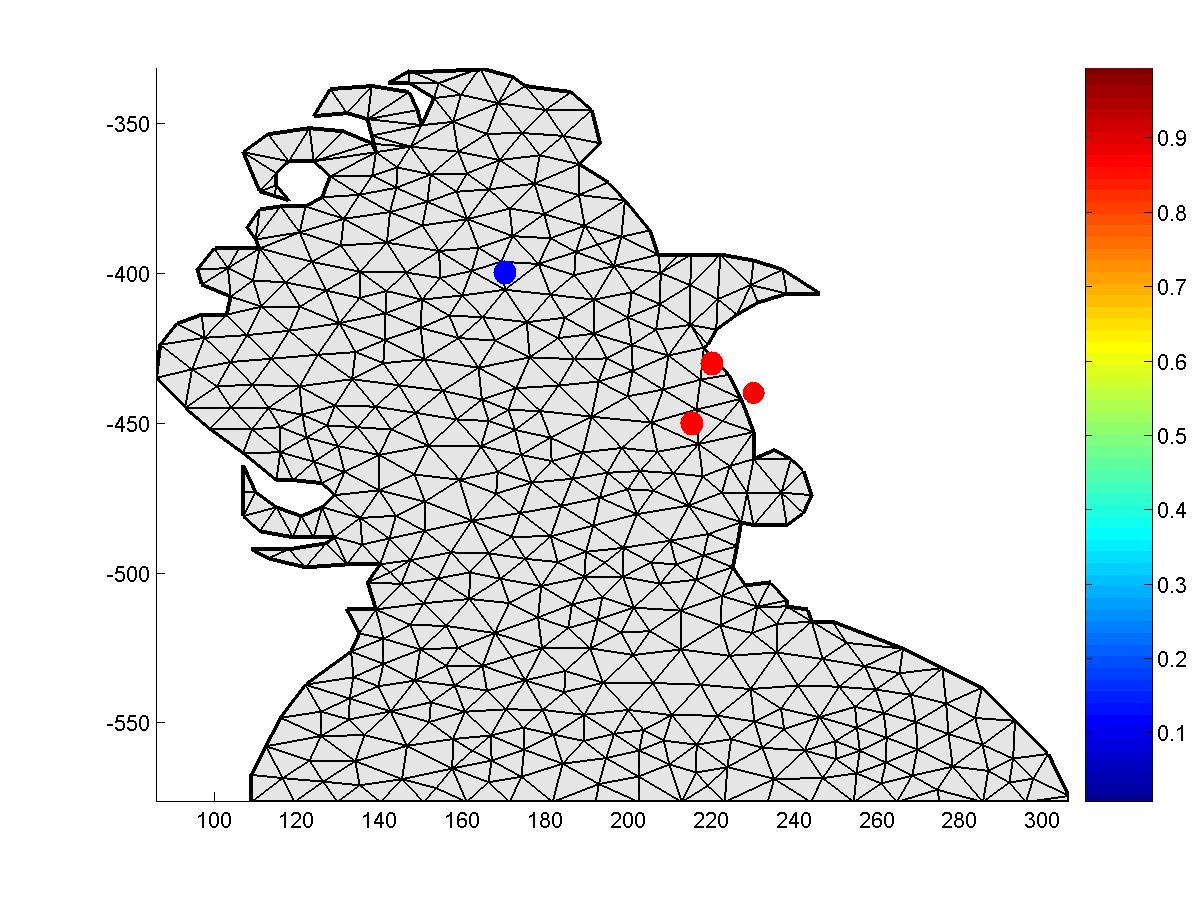
\includegraphics[height=7cm]{casta}
\end{figure}

\normalsize{(last modified: April~2015)}

\vfill

\parbox{.20\textwidth}{
\flushleft

\includegraphics[height=1.75cm]{gherlogo.PNG}
}\parbox{.60\textwidth}{
\centering
\vspace{.4cm}


\footnotesize{GeoHydrodynamics and Environment Research, MARE\\ 
Departement of Astrophysics, Geophysics and Oceanography\\
University of Li\`{e}ge\\ 
\url{http://modb.oce.ulg.ac.be}
}
\vspace{.15cm}
}\parbox{.20\textwidth}{
\flushright

\includegraphics[height=1.75cm]{logo_ulg.PNG}
}

\end{center}

\end{titlepage}

%%----------------------
%\newpage
%
%\thispagestyle{empty}
%
%\vspace{5cm}



% \input{DivaModif} contains the additionnal documents

%--------------------------------------
\dominitoc
\setcounter{tocdepth}{1}
\tableofcontents

\mainmatter
\pagestyle{fancy}

\chapter{Error fields}

\section{Use of error maps}

See documentation for the general theory on error calculations and the different approximative versions implemented. For practical use, one has to be aware that
\begin{itemize}
\item The error fields are only indicative as their reliability depend on the reliability of the statistical parameters used
\item The error field in the netCDF file \file{result.nc} is the standard deviation, not the error variance.
\item The parameter varbal in \file{param.par} controls the overall amplitude of this error field, the structure being controlled by the data distribution (not their value).
\item When varkak=1 the error field contains thus rather relative errors since to get a error standard deviation one would need to mulitply by the square root of the error variance of the first guess (or in other word, the error variance associated with the background field).
\item With varbak=1 the field is of course easily used to mask regions where the analysis has used no data as in these regions the analysis error standard deviation approaches 1 whereas in regions with good coverage and data quality the value will be close to zero.
\item With parameter optimisations varbak is normally estimated from the data but as the other parameters (L and SN) the estimate must be supervised
\end{itemize}

Examples with scalings by varbak


\clearpage

%------------------------------------
\section{Integrals over (sub-)domains}
%------------------------------------

Very often, we are not only interested in the analysed field itself but also in its integral over the
total domain or a sub-domain. If we have the analysis on a sufficiently fine output grid, the integral
itself is then just a sum of the values at the grid points covering the integration domain, multiplied by the
grid-cell surface. 

We do not consider here the additional approximation brought by replacing a continuous integral by
a discrete sum. Indeed, generally the output grid is fine compared to the scales of interest
and the sum can be considered an "exact" integral. Hence, we will focus on the error on a discrete sum of the analysed field.

An application of this theory is found in \citet{YARI12}, where the authors estimated transports through the Strait of Otranto (Adriatic Sea) using \diva and the calculation of integrals.

\subsection{Theory}
%------------------

Formally, if $\mathbf{x}^a$ is a column vector containing the analysed field values at the grid
points defining the integration domain, the weighted sum $I$ over this values is
\begin{equation}
I~=~\transp{(\mathbf{x}^a)} \mathbf{h}
\end{equation}
where $\transp{\quad}$ stands for the transposed vector or matrix and $\mathbf{h}$ is a column vector of the same size as
$\mathbf{x}^a$ but whose components are the weight associated with each integration point. The weight is typically the surface associated with
the integration point. For an integration over a uniform grid, the weights can without loss of generality be unit (the surface dimension can be retrieved at the end by global multiplication). 

Note that the weights here have nothing to do with the weight on data points for an analysis\index{Weight}.

Now the analysis is not exact but has an associated random error $\mathbf{\epsilon}^a$ with respect to the true
field values $\mathbf{x}^t$:

\begin{equation}
{\mathbf{x}^a} = \mathbf{x}^t + \mathbf{\epsilon}^a
\end{equation}
On statistical average (noted $< \quad >$), we suppose the analysis is unbiased and
\begin{equation}
<{\mathbf{x}^a}> = \mathbf{x}^t 
\end{equation}
In order to calculate the error variance on the sum, we calculate the expected square distance with respect to the true sum:
\begin{equation}
\Delta^2 = < \transp{\mathbf{h}}( {\mathbf{x}^a} - \mathbf{x}^t) \transp{({\mathbf{x}^a} - \mathbf{x}^t )} \mathbf{h} > = \transp{\mathbf{h}} \, \mathbf{P}^a \, \mathbf{h}
\label{eq:errorintegral}
\end{equation}
where $\mathbf{P}^a = <\mathbf{\epsilon}^a \transp{\mathbf{\epsilon}^a} >$ is the error-covariance matrix of the analysis.
We see that the spatial covariances of the analysis-error field are required to calculate the error variance on $I$. Since this
covariance matrix is not diagonal, it is not sufficient to sum up the local error values of the error fields of $\mathbf{x}^a$. The latter sum would limit
the double sum of \eqref{eq:errorintegral} to the diagonal terms of $\mathbf{P}^a$.


\subsection{Implementation}
Exploiting the equivalence of \diva and OI, we know that

\begin{equation}
\mathbf{P}^a ~=~ \mathbf{P} -  \transp{\mathbf{C}} \left( \mathbf{B}+\mathbf{R} \right)^{-1} \mathbf{C}
\label{eq:covariance}
\end{equation}
where $\mathbf{P}$ is the covariance matrix (size $N_g\times N_g$) of the background field between the $N_g$ grid points under consideration, $\mathbf{B}$ 
the covariance matrix (size $N_d \times N_d$) of the background field between the $N_d$ data points, $\mathbf{C}$  is the
 covariance matrix (size $N_d \times N_g$) of the background field between the  data points and grid points and finally $\mathbf{R}$ is the error covariance matrix (size $N_d \times N_d$) on the data.
 
We could calculate the covariances matrices involved exactly (as done for the exact error calculation) and then calculate \eqref{eq:errorintegral} but this would be prohibitively expensive if done in a brute force approach. However when done in a clever way it is feasible.

\subsubsection{Direct approach}

Using \eqref{eq:covariance} and \eqref{eq:errorintegral} we can write

 \begin{equation}
 \Delta^2 = \transp{\mathbf{h}}\, \mathbf{P} \, \mathbf{h} - \transp{\mathbf{h}} \underbrace{\transp{\mathbf{C}} \left( \mathbf{B}+\mathbf{R} \right)^{-1}} \, \underbrace{\mathbf{C}  \, \mathbf{h}}
 \label{eq:totalerror}
 \end{equation}
 
The term $\mathbf{C}  \, \mathbf{h}$ is readily interpreted as a columns vector containing $N_d$ elements. Element $j$ is the (weighted) sum of the covariances of all integration points with the data point $j$. The middle term is the analysis operator that provides the analysis on the grid points when providing on input a columns vector of size $N_d$. Hence the recipe to calculate $\Delta^2$ without explicitly forming the error-covariance matrices is the following:
\begin{itemize}
\item Perform a double sum on all covariances between grid points to calculate $\transp{\mathbf{h}} \, \mathbf{P} \, \mathbf{h}$.
\item For the term to subtract, evaluate it starting from the right: form a pseudo-data vector by summing covariances of all grid points with each data point, analyse it and finally sum up the analysis at the grid points.
\end{itemize}

All we have to to is to be calculate covariance functions. This can be done with the module {\tt covar} of \diva, which allows one to calculate
a series of covariances with a single matrix inversion. Hence the recipe of calculating \eqref{eq:totalerror} includes a \diva run to calculate covariances (cost roughly equal to an analysis with full error field), followed by a second \diva run to analyse the "data" $\mathbf{C}  \, \mathbf{h}$.



\subsubsection{Hybrid approach}

A simplified version can be used, using to some extend the fact the covariance functions in an infinite domain are known analytically when no
advection constraint or variable correlation length is activated. We can indeed introduce an approximation that makes the calculation manageable without calculating the covariances with \diva itself. Instead of using the exact covariances on the background field, we use the covariances we would find in an infinite domain with constant correlation length and without advection constraint. In this case, we know
that the correlation function $c$ between two points is
\begin{equation}
c(r) ~=~{r \over L} K_1 \left(r \over L\right)
\end{equation}
where $r$ is the distance between the two points, $L$ the correlation length and $K_1$ a Bessel function\index{Bessel function}. To get the covariance function we simply have to multiply by the variance $\sigma^2$ of the background field.

This way we can estimate $\Delta^2$ by calculating these covariance functions between grid and data points and performing one analysis with \diva.

\subsubsection{Inflation approach}

A second simplified approach makes even stronger assumptions but shows how we can try to "extrapolate" the error estimated from the sum of the diagonal terms of $\mathbf{P}^a$ to the estimation of the double sum. To do so, we assume that the analysis error has a spatial correlation scale similar to the analysis. Even better, we showed in paper that with L/ ????
This is probably too severe and we will therefore overestimate the integral error. 
Here we use a continuous formulation to calculate an approximation of $\Delta$ noted $\tilde{\Delta}$ by starting from the sum expressed as continuous integral
\begin{equation}
{\Delta}^2= {1 \over \Delta x^2 \Delta y^2} \int_D \int_D <{\epsilon}^a(\vect{x}) {\epsilon}^a(\vect{x}^\prime)> d \vect{x}^\prime d \vect{x} 
\end{equation}
where $\vect{x}$ and $\vect{x}^\prime$ stand for positions in the domain of integration $D$. When we suppose the covariance is isotropic and note $r$ the distance between points
$\vect{x}$ and $\vect{x}^\prime$ we have 
\begin{equation}
{\Delta}^2= {1 \over \Delta x^2 \Delta y^2} \int_D \int_D <{\epsilon}^a(\vect{x}) {\epsilon}^a(\vect{x}) > c(r) d \vect{x}^\prime d \vect{x}  
\end{equation}
which we can evaluate in polar coordinates the inner integral expanded to infinity to find an approximate value
\begin{equation}
\tilde{\Delta}^2= {2 \pi \over \Delta x^2 \Delta y^2} \int_D <{\epsilon}^a(\vect{x}) {\epsilon}^a(\vect{x}) > \int_0^{\infty}  r c(r) d r \, d \vect{x}
\end{equation}
with the Bessel function for the correlation function $c$ this yields
\begin{equation}
\tilde{\Delta}^2= {4 \pi L^2 \over \Delta x^2 \Delta y^2} \int_D <{\epsilon}^a(\vect{x}) {\epsilon}^a(\vect{x}) >  d \vect{x}
\end{equation}

If we had used the naive approach of neglecting the spatial covariances, the double sum would have been restricted to a simple sum on diagonal and we would calculated the underestimated error 
\begin{equation}
\tilde{\tilde{\Delta}}^2= {1 \over \Delta x \Delta y} \int_D <{\epsilon}^a(\vect{x}) {\epsilon}^a(\vect{x}) >  d \vect{x}.
\end{equation}
Hence we see that we should apply an inflation factor of $\sqrt{{4 \pi L^2 \over \Delta x \Delta y}}$ on $\tilde{\tilde{\Delta}}$ to get a better estimate of the error standard deviation. In practice this inflation factor is probably a little too high (we assumed the analysis error to have the same correlation length as the analysis while in reality it is generally smaller and we extended one of the integrals to an infinite domain, adding up more errors).

1.70677 (see paper in JTECH)

So theoretical factor to be applied: 

Receipe:

standart deviation on the subdomain  average= 1.44 \sqrt{L^2 \over \delta x \delta y} \sqrt{\sum_S \epsilon^2 \over \sum_S} 

where $L$ is the correlation length scale of the analysis and epsilon the standard deviation found in the error field. 

Compare with direct method and show example on synthetic data set and later on Calamus

\subsection{Use for EMODNET}


The full approach was implemented into \command{divaintegral} see general user manual.

In the scope of EMODNET, there is no need to go into the cost of this calculation as error fields themselves are only approximate.

Also if the subdomain is changed, the full method would need a recalculation by diva and cannot perform the calculation on a final product.

 Hence the simple inflation method can be used instead and allows redefining subregions at any moment.

For this, there must be a netCDF file \file{subdomain.nc} containing a mask of 1 and 0 on exactly the same grid as results.nc (From contours to mask etc in R probably).

Then running \command{dvmean} will calculate the mean value and the standard deviation of the mean.

\chapter{Environmental predictors and constraints}


\section{Background information and habitats}
Use of bottom depth to create mask of potential occurence. In other regions use small RL so that no information is propagated into these parts



Creating mask for selection of topographic regions

Creation of RL based on habitats ?

Creation of background fields from MexENT ?


\end{document}